\documentclass[10pt,a4paper]{scrartcl}
\setkomafont{disposition}{\normalfont\bfseries}
\usepackage[utf8]{inputenc}
\usepackage[french]{babel}
\usepackage[T1]{fontenc}
\usepackage{amsmath}
\usepackage{amsthm}
\usepackage{amsfonts}
\usepackage{amssymb}
\usepackage{graphicx}
\usepackage{mathrsfs}
\usepackage{url}
\usepackage{color}
\usepackage{hyperref}
\usepackage{cleveref}
\usepackage{listings}
\definecolor{mygreen}{RGB}{28,172,0} % color values Red, Green, Blue
\definecolor{mylilas}{RGB}{170,55,241}
\lstset{
language=R,
basicstyle=\scriptsize\ttfamily,
commentstyle=\ttfamily\color{green},
numbers=left,
numberstyle=\ttfamily\color{black}\footnotesize,
stepnumber=1,
numbersep=5pt,
backgroundcolor=\color{white},
showspaces=false,
showstringspaces=false,
showtabs=false,
frame=single,
tabsize=2,
captionpos=b,
breaklines=true,
breakatwhitespace=false,
keywordstyle=\color{blue},
stringstyle=\color{magenta},
literate=
  {á}{{\'a}}1 {é}{{\'e}}1 {í}{{\'i}}1 {ó}{{\'o}}1 {ú}{{\'u}}1
  {Á}{{\'A}}1 {É}{{\'E}}1 {Í}{{\'I}}1 {Ó}{{\'O}}1 {Ú}{{\'U}}1
  {à}{{\`a}}1 {è}{{\`e}}1 {ì}{{\`i}}1 {ò}{{\`o}}1 {ù}{{\`u}}1
  {À}{{\`A}}1 {È}{{\'E}}1 {Ì}{{\`I}}1 {Ò}{{\`O}}1 {Ù}{{\`U}}1
  {ä}{{\"a}}1 {ë}{{\"e}}1 {ï}{{\"i}}1 {ö}{{\"o}}1 {ü}{{\"u}}1
  {Ä}{{\"A}}1 {Ë}{{\"E}}1 {Ï}{{\"I}}1 {Ö}{{\"O}}1 {Ü}{{\"U}}1
  {â}{{\^a}}1 {ê}{{\^e}}1 {î}{{\^i}}1 {ô}{{\^o}}1 {û}{{\^u}}1
  {Â}{{\^A}}1 {Ê}{{\^E}}1 {Î}{{\^I}}1 {Ô}{{\^O}}1 {Û}{{\^U}}1
  {œ}{{\oe}}1 {Œ}{{\OE}}1 {æ}{{\ae}}1 {Æ}{{\AE}}1 {ß}{{\ss}}1
  {ű}{{\H{u}}}1 {Ű}{{\H{U}}}1 {ő}{{\H{o}}}1 {Ő}{{\H{O}}}1
  {ç}{{\c c}}1 {Ç}{{\c C}}1 {ø}{{\o}}1 {å}{{\r a}}1 {Å}{{\r A}}1
  {€}{{\EUR}}1 {£}{{\pounds}}1
}

\lstset{language=Matlab,%
%basicstyle=\color{red},
breaklines=true,%
morekeywords={matlab2tikz},
keywordstyle=\color{blue},%
morekeywords=[2]{1}, keywordstyle=[2]{\color{black}},
identifierstyle=\color{black},%
stringstyle=\color{mylilas},
commentstyle=\color{mygreen},%
showstringspaces=false,%without this there will be a symbol in the places where there is a space
numbers=left,%
numberstyle={\tiny \color{black}},% size of the numbers
numbersep=9pt, % this defines how far the numbers are from the text
emph=[1]{for,end,break},emphstyle=[1]\color{red}, %some words to emphasise
%emph=[2]{word1,word2}, emphstyle=[2]{style},    
}
\lstset{literate=
{á}{{\'a}}1 {é}{{\'e}}1 {í}{{\'i}}1 {ó}{{\'o}}1 {ú}{{\'u}}1
{Á}{{\'A}}1 {É}{{\'E}}1 {Í}{{\'I}}1 {Ó}{{\'O}}1 {Ú}{{\'U}}1
{à}{{\`a}}1 {è}{{\`e}}1 {ì}{{\`i}}1 {ò}{{\`o}}1 {ù}{{\`u}}1
{À}{{\`A}}1 {È}{{\'E}}1 {Ì}{{\`I}}1 {Ò}{{\`O}}1 {Ù}{{\`U}}1
{ä}{{\"a}}1 {ë}{{\"e}}1 {ï}{{\"i}}1 {ö}{{\"o}}1 {ü}{{\"u}}1
{Ä}{{\"A}}1 {Ë}{{\"E}}1 {Ï}{{\"I}}1 {Ö}{{\"O}}1 {Ü}{{\"U}}1
{â}{{\^a}}1 {ê}{{\^e}}1 {î}{{\^i}}1 {ô}{{\^o}}1 {û}{{\^u}}1
{Â}{{\^A}}1 {Ê}{{\^E}}1 {Î}{{\^I}}1 {Ô}{{\^O}}1 {Û}{{\^U}}1
{œ}{{\oe}}1 {Œ}{{\OE}}1 {æ}{{\ae}}1 {Æ}{{\AE}}1 {ß}{{\ss}}1
{ű}{{\H{u}}}1 {Ű}{{\H{U}}}1 {ő}{{\H{o}}}1 {Ő}{{\H{O}}}1
{ç}{{\c c}}1 {Ç}{{\c C}}1 {ø}{{\o}}1 {å}{{\r a}}1 {Å}{{\r A}}1
{€}{{\euro}}1 {£}{{\pounds}}1 {«}{{\guillemotleft}}1
{»}{{\guillemotright}}1 {ñ}{{\~n}}1 {Ñ}{{\~N}}1 {¿}{{?`}}1
}
\usepackage[french,onelanguage,ruled,lined,linesnumbered]{algorithm2e}
\SetKw{And}{et}
\SetKw{From}{allant de}
\author{\textsc{BOUCETTA I.} \& \textsc{TRAN Q.N.H.} \& \textsc{WARTELLE A.}}
\title{Rapport de projet OS10}
\subtitle{Etude de l'algorithme GRASP pour le problème d'ordonnancement FJSSP-nfa}
\date{\today}

\begin{document}
\maketitle
\renewcommand{\contentsname}{Sommaire}
\tableofcontents
\clearpage

\begin{abstract}
Ce travail a pour objectif d'étudier l'article de 2010 de Rajkumar, Muthukannan \& Asokan, P \& Vamsikrishna, V.
portant sur un algorithme de recherche locale randomisée : \emph{Greedy Randomized Adaptive Search Procedure} (GRASP),
dans le cadre d'un problème de job shop : le \emph{Flexible Job Shop Scheduling Problem with non fixed-availability constraints}
(FJSSP-nfa) \cite{GRASP}. 
Cette extension du problème du job shop permet de prendre en compte deux aspects importants de la production :
\begin{enumerate}
\item la flexibilité des machines pour effectuer des opérations, c'est-à-dire qu'une opération n'aura pas une machine
prédéfinie à l'avance pour son exécution, on aura en effet le choix entre plusieurs machines avec différents temps
d'exécution associés. Cette diversité des temps d'exécution est en général lié au temps de préparation d'une
pour le traitement d'une opération donnée mais surtout à la performance et à l'adéquation de la machine
pour exécuter une telle tâche
\item la prise en compte de tâches de maintenance à effectuer dans des fenêtres de temps données (non fixité). En effet
les machines ont besoin d'être entretenues afin d'éviter (si possible) des pannes ou des défaillances. Durant une
tâche de maintenance, une machine est indisponible est ne peut pas traiter d'opération, ce qui impacte fortement
les performances d'une affectation d'opérations et d'ordonnancement de celles-ci.
\end{enumerate}
Avec la prise en compte de la flexibilité des machines, le FJSSP-nfa permet de travailler sur de nouveaux
critères portant de la charge de travail, c'est à dire sur le temps d'utilisation de chaque machine qui
n'est plus fixé comme dans le cas d'un CJSSP. Ainsi le FJSSP-nfa est un problème multi-critère portant
sur la charge de travail totale et maximal des machines et sur le makespan de l'ordonnancement (temps
de complétion maximale).
Enfin le problème de job shop classique étant déjà NP-difficile, le FJSSP-nfa l'est aussi.
De plus, avec les difficultés rajoutées par la flexibilité des machines et la maintenance,
une approche de résolution par méthode exacte est semble presque inenvisageable\footnote{d'après \cite{GA1},
les méthodes exactes par graphes disjonctifs sont actuellement limités à 20 jobs et 10 machines pour
le FJSSP (sans maintenance)}. Ainsi ce sont les heuristiques comme l'algorithme GRASP (\cite{GRASP}) 
et les méta-heuristiques comme les algorithmes génétiques(\cite{GA1},\cite{GA2}) qui ont rencontré le plus de succès.

\end{abstract}

\section{Introduction}

Avec la notation de Graham, ce problème peut s'écrire sous la forme : 
\[J_{m}|flexibility,nfa|W_{tot},W_{max},C_{max}\].
On ainsi un ensemble de job i
Une solution à ce problème doit indiquer les affectations de chaque opération à une machine ainsi
que les les temps de complétions (ou de début) de chaque opération
et de chaque tâche de maintenance (et de chaque job et chaque machine).
En eff
%Il s'agit d'une extension FJSSP avec des contraintes de tâches de maintenance à exécuter sur une fenêtre de temps
%pour chaque machine.
%Le FJSSP est lui-même une extension du problème de job shop classique (CJSSP) où les opérations des jobs peuvent être
%exécutés, de manière non-préemptive et ordonnée, sur différentes machines. Ainsi, pour transformer un FJSSP en un
%CJSSP, il faut affecter une machine à chaque opération \footnote{il s'agit d'un  
%\emph{Operation Machine Affectation Problem (OMAP)}} de telle sorte à minimiser
%la charge (temps d'occupation par les opérations et les tâches de maintenances) totale de chaque machine $W_{tot}$
%et la charge maximale $W_{tot}$.
%Ce problème d'affectation peut-être résolu de 2 manières avec le problème d'ordonnancement :
%\begin{enumerate}
%\item de manière hiérarchique en résolvant d'abord le problème d'affectation
%\item de manière conjointe avec une approche intégrée
%\end{enumerate}
%  ou de manière h
%
%\begin{algorithm}[H]
%    \caption{Algorithme PPI : Plus proche insertion}
%    
%    \tcp{Déclaration et Initialisation}
%     $C_{min}$ : Coût minimal d'insertion
%     
%     $D_{min} \leftarrow +\infty$ : Distance minimale au circuit
%     
%     $\forall i=1...n,D_{tour}^{i} \leftarrow +\infty$, : Distances des nœuds encore à insérer au circuit
%     
%     $B$ : Nœud sélectionné à insérer (B pour "Best")
%     
%     $A \leftarrow 0$ : Nœud d'insertion de coût minimal (A avant B, ou B voisin de A)
%     
%    \tcp{Recherche du ième point du point à ajouter au chemin actuel}
%    \For{$i$ \From $1$ \KwTo $N$}{
%    
%        \tcp{Réinitialiser le coût et la distance minimales}
%        $C_{min} \leftarrow +\infty$
%        
%        $D_{min} \leftarrow +\infty$
%        
%        \tcp{Recherche parmi les nœuds qui ne sont pas encore dans le circuit}
%        \For{$j$ \From $1$ \KwTo $N$}{
%            \If{$j \notin circuit$}{
%            Recalculer la distance $D_{tour}^{j}$ du nœud j au circuit en prenant en compte le (i-1)-ème nœud ajouté (nœud $i-1$ du circuit)
%            
%            Mise à jour de la distance minimale : $D_{min} \leftarrow min(D(B,node(i-1)) ,D(j,node(i-1)))$
%           
%            
%            Mise à jour du meilleur nœud à ajouter : $B \leftarrow arg1min(D(B,node(i-1)) ,D(j,node(i-1)))$  \footnote{node(i-1) est l'index du (i-1)-ème nœud ajouté au circuit et D(,) est la distance entre deux nœuds}
%             }
%            
%	        \If{$j \in circuit$}{
%	        Calculer le coût d'ajout $C_{j}$ de B après le nœud j  dans le circuit
%	        
%	        
%	        Mise à jour du coût (minimal) de meilleure insertion : $C_{min} \leftarrow min(C_{A},C_{j})$
%	        
%	        Mise à jour du nœud (prédécesseur) de meilleure insertion : $A \leftarrow argmin(C_{A},C_{j})$
%	        }
%        }
%        Ajouter le nœud B à la suite du nœud A dans le circuit.
%    }
%\end{algorithm}
\begin{algorithm}
  \caption{Assigner les opérations aux machines (\emph{routing})}
  \label{algo:routing}
  \tcp{Initialisation}
  $t$ le nombre de solutions\;
  $A = \{\alpha_1, \alpha_2,..., \alpha_t\}$ l'ensemble des valeurs $\alpha$ discrètes aléatoires telle que $0 \leq \alpha_i \leq 1 \, \forall i = \overline{1,t}$\;
  $S = \{s_1, s_2,..., s_t\}$ l'ensemble des solutions à construire\;
  \tcp{Assignement}
  \ForEach{$\alpha_i \in A$}{
    $\sigma$ l'ensemble des opérations non assignées\;
    $s_i$ la solution à construire\;
    $s_i \leftarrow \emptyset$\;
    \While{$\sigma \neq \emptyset$}{
      Chercher $o_M$ l'opération dont le processing time est le plus longue\;
      Chercher $o_m$ l'opréation dont le processing time est le plus court\;
      $Range \leftarrow p_{o_M} - p_{o_m}$\;
      $Width \leftarrow Range * \alpha_i$\;
      Construire RCL l'ensemble des opérations non assignées $o \in \sigma$ telle que $p_{o_m} \leq p_o \leq p_{o_m} + Width$\;
      Ordonner RCL dans l'ordre croissant de processing time\;
      Pondérer les éléments de RCL par la fonction linéaire $\frac{1}{r}$ où $r$ est l'ordre de l'élément\;
      Choisir de manière aléatoire un élément $o^*$ de RCL en tenant compte des pois ci-dessus\;
      $s_i \leftarrow s_i \cup o^*$\;
      $\sigma \leftarrow \sigma \backslash o^*$\;
    }
    Calculer la charge totale de $s_i$\;
  }
\end{algorithm}

\begin{algorithm}
  \caption{Ordonner les opérations et les maintenances sur les machines (\emph{scheduling})}
  \label{algo:scheduling}
  \tcp{Initialisation}
  $t$ le nombre de solutions (fixé à l'algorithme \eqref{algo:routing}) \;
  $A = \{\alpha_1, \alpha_2,..., \alpha_t\}$ l'ensemble des valeurs $\alpha$ discrètes aléatoires telle que $0 \leq \alpha_i \leq 1 \, \forall i = \overline{1,t}$ (pas forcément identique à l'algorithme \eqref{algo:routing})\;
  $S = \{s_1, s_2,..., s_t\}$ l'ensemble des solutions à construire\;
  \tcp{Ordonnancement}
  \ForEach{$\alpha_i \in A$}{
    $\sigma$ l'ensemble des opérations non ordonnées\;
    $s_i$ la solution à ordonner\;
    $s_i \leftarrow \emptyset$\;
    \While{$\sigma \neq \emptyset$}{
      Chercher $o_M$ l'opération dont le processing time est le plus longue; et $o_m$ l'opréation dont le processing time est le plus court en tenant compte les maintenances qui doivent être situées au milieu des intervalles donnés $\left[t_{jl}^E, t_{jl}^L\right]$ \;
      $Range \leftarrow p_{o_M} - p_{o_m}$\;
      $Width \leftarrow 1 + Range * \alpha_i$\;
      Construire RCL l'ensemble des opérations non assignées $o \in \sigma$ telle que $p_{o_m} \leq p_o \leq p_{o_m} + Width$\;
      Ordonner RCL dans l'ordre croissant de processing time\;
      Pondérer les éléments de RCL par la fonction linéaire $\frac{1}{r}$ où $r$ est l'ordre de l'élément\;
      Choisir de manière aléatoire un élément $o^*$ de RCL en tenant compte des pois ci-dessus\;
      Ordonner $o^*$ en tenant compte la date de disponibilité la plus tôte et les maintenances\;
      $\sigma \leftarrow \sigma \backslash o^*$\;
    }
    Ordonner les maintenances au milieu des intervalles donnés $\left[t_{jl}^E, t_{jl}^L\right]$ sans collision avec les opérations scédulées\;
    Calculer le makespan de $s_i$\;
  }
\end{algorithm}

\section{Résultats et comparaisons}
%
%\begin{figure}[!ht]
%    \centering
%    \includegraphics[width=0.8\linewidth]{img/PPI1.png}
%    \caption{Chemin de l'algorithme PPI}
%    \label{PPI1}
%\end{figure}
\subsection{Spécification de l'ordinateur}
Nous tournons le code sur un ordinateur portable de processeur Intel(R) Core(TM) i7-7700HQ CPU\@2.8GHz (8 CPUs), 8 Go de RAM. Le programme est compilé par Visual Studio Code 2017. Le générateur choisi est \texttt{MersenneTwister.h} (v1.0, 15/05/2003).

\subsection{Résultats et comparaisons avec ceux de l'article}
Nous réalisons $1000$ solutions (itérations) séquentiellement parmi lesquelles nous choissions les meilleurs corresponsdant au triplet voulu.
\begin{table}[!h]
  \centering
  \begin{tabular}{|c|c|c|}
    \hline
    Critères & Valeurs de l'article & Nos valeurs \\
    \hline
    $W_t$ & 103 & 103 \\
    $W_{max}$ & 16 & 15 \\
    $C_{max}$ & 18 & 13 \\
    $F(0.5;0.3;0.2)$ & 59.9 & 60.1 \\
    $F(0.5;0.2;0.3)$ & 60.1 & 60.4 \\
    \hline
  \end{tabular}
  \caption{Résultat pour problème $8 \times 8$}
\end{table}

\begin{table}[!h]
  \centering
  \begin{tabular}{|c|c|c|}
    \hline
    Critères & Valeurs de l'article & Nos valeurs \\
    \hline
    $W_t$ & 60 & 60 \\
    $W_{max}$ & 7 & 8 \\
    $C_{max}$ & 9 & 11 \\
    $F(0.5;0.3;0.2)$ & 33.9 & 35.4 \\
    $F(0.5;0.2;0.3)$ & 34.1 & 35.6 \\
    \hline
  \end{tabular}
  \caption{Résultat pour problème $10 \times 10$}
\end{table}

\begin{table}[!h]
  \centering
  \begin{tabular}{|c|c|c|}
    \hline
    Critères & Valeurs de l'article & Nos valeurs \\
    \hline
    $W_t$ & 107 & 98 \\
    $W_{max}$ & 13 & 14 \\
    $C_{max}$ & 16 & 20 \\
    $F(0.5;0.3;0.2)$ & 60.3 & 57.2 \\
    $F(0.5;0.2;0.3)$ & 60.9 & 57.8 \\
    \hline
  \end{tabular}
  \caption{Résultat pour problème $15 \times 10$}
\end{table}

\begin{table}[!h]
  \centering
  \begin{tabular}{|c|c|c|}
    \hline
    Critères & Valeurs de l'article & Nos valeurs \\
    \hline
    $W_t$ & 40 & 40 \\
    $W_{max}$ & 9 & 9 \\
    $C_{max}$ & 16 & 13 \\
    $F(0.5;0.3;0.2)$ & 25.9 & 26 \\
    $F(0.5;0.2;0.3)$ & 26.6 & 26.5 \\
    \hline
  \end{tabular}
  \caption{Résultat pour problème $4 \times 5$}
\end{table}

Nos valeurs sont très proche celles trouvées dans l'articles, particulièrement certaines sont meilleures, signifiant la reproductivité facile de l'algorithme. Son application aura peu de dépendance de l'ordinateur de planification au niveau de résultat.

D'autre part, au niveau de temps d'exécution, qui joue un rôle important de chaque algorithme, leurs déroulement ne prennent pas plus de \emph{2 seconds} (figure \eqref{tab:temps_exec}). Autrement dit, l'algorithme GRASP est efficace contre le problème de type FJSSP-nfa.

\begin{table}[!h]
  \centering
  \begin{tabular}{|c|c|c|}
    \hline
    Problème & Temps d'exécution (ms) \\
    \hline
    $4 \times 5$ & 28.6767 \\
    $8 \times 8$ & 150.71 \\
    $10 \times 10$ & 427.403 \\
    $15 \times 10$ & 1661.43 \\
    \hline
  \end{tabular}
  \caption{Temps d'exécution de chaque problème exemplaire}
  \label{tab:temps_exec}
\end{table}

Les ordonnancements finaux pour chaque problème exemplaire sont inclus dans l'annexe \eqref{annexe:visual_ordo}.

\section{Annexes}

\subsection{Visualisation de tournées (plots.m)}
\lstinputlisting[language=Matlab]{src/plotJob.m}

\subsection{Automatisation de traçage des exemplaires (tests.m)}
\lstinputlisting[language=Matlab]{src/tests.m}

\subsection{Visualisation de statistiques (stats.R)}
%\lstinputlisting[language=R]{stats.R}

\subsection{Visualisation des ordonnacements}
\label{annexe:visual_ordo}
\begin{figure}
  \centering
  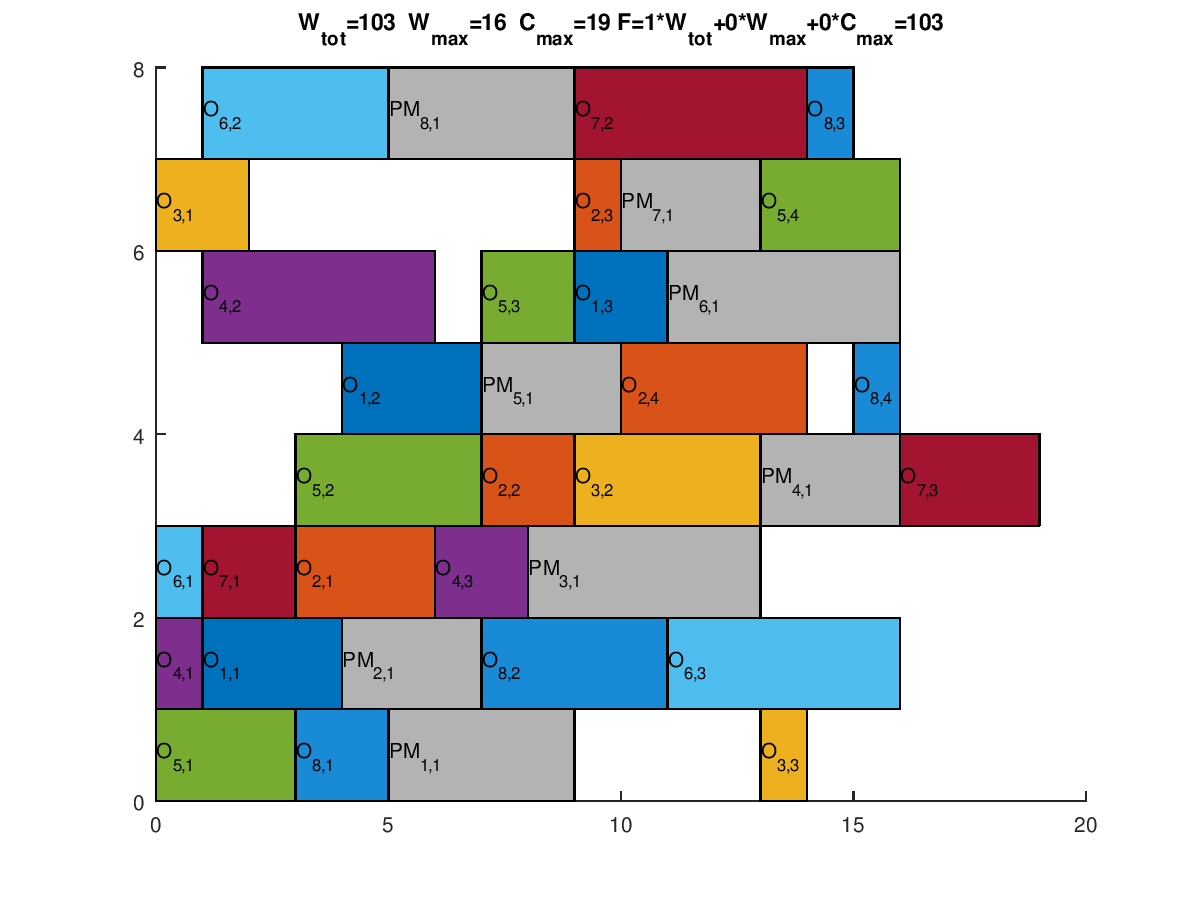
\includegraphics[width=0.8\textwidth]{img/results8x8_Wtot.png}
  \caption{$8 \times 8$ $W_{t}$ : $(W_t, W_{max}, C_{max}) = (40; 17; 17)$}
\end{figure}
\begin{figure}
  \centering
  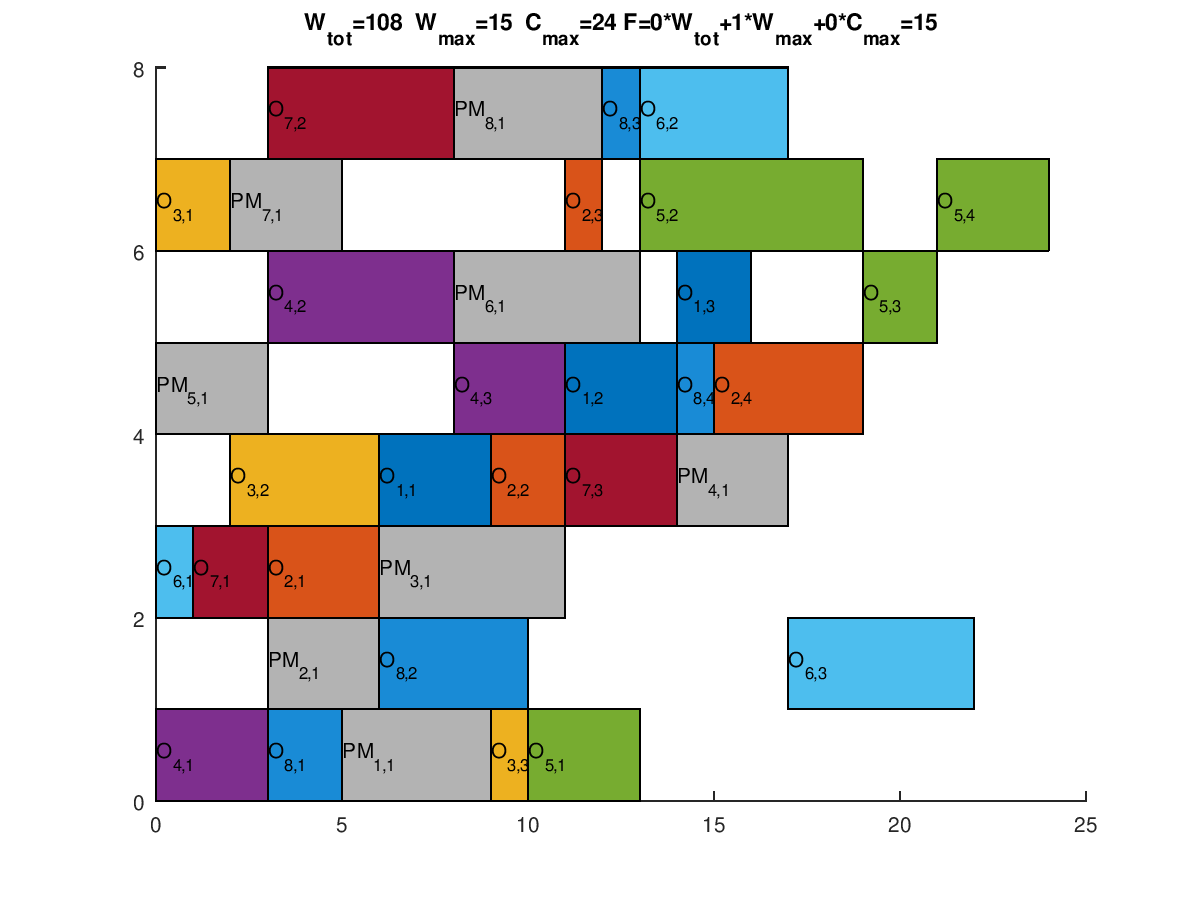
\includegraphics[width=0.8\textwidth]{img/results8x8_Wmax.png}
  \caption{$8 \times 8$ $W_{max}$ : $(W_t, W_{max}, C_{max}) = (41; 9; 18)$}
\end{figure}
\begin{figure}
  \centering
  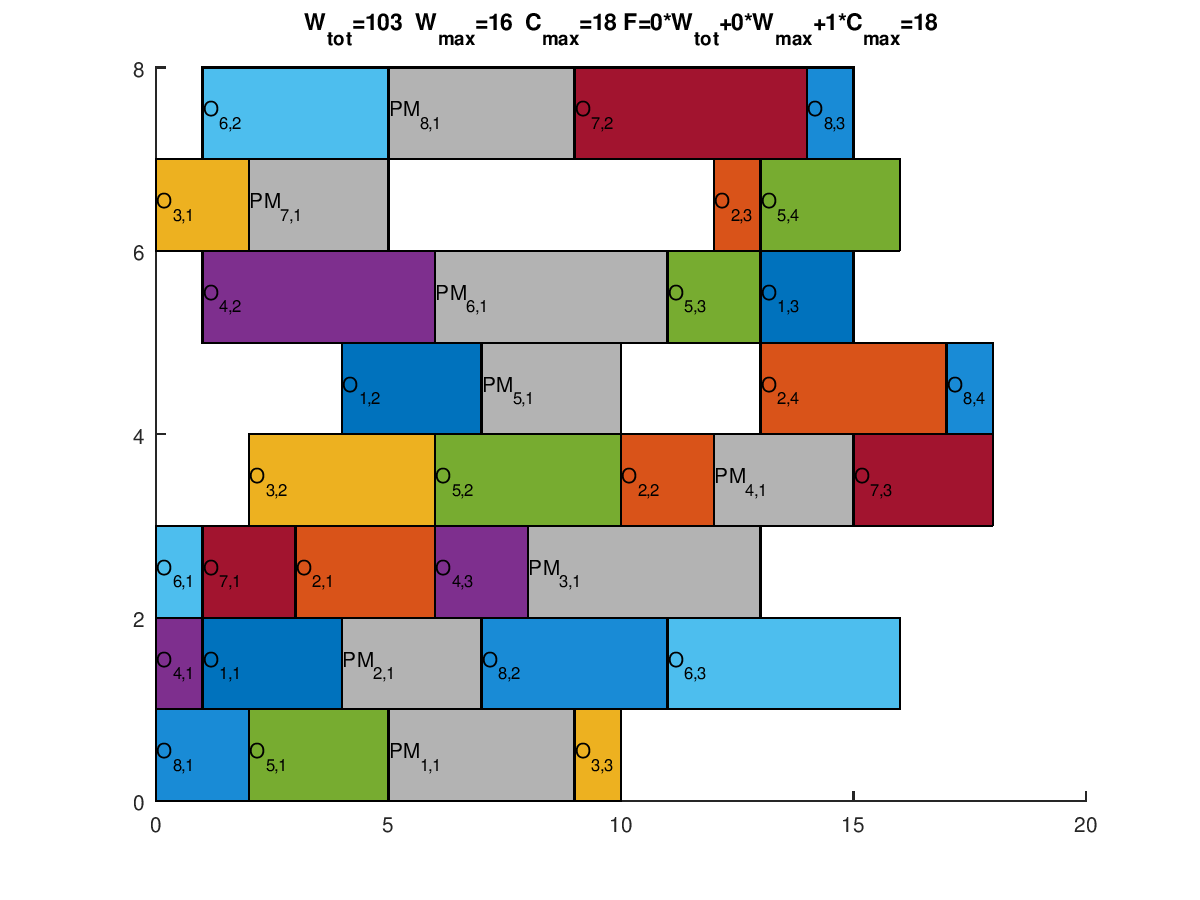
\includegraphics[width=0.8\textwidth]{img/results8x8_Cmax.png}
  \caption{$8 \times 8$ $C_{max}$ : $(W_t, W_{max}, C_{max}) = (105; 16; 19)$}
\end{figure}
\begin{figure}
  \centering
  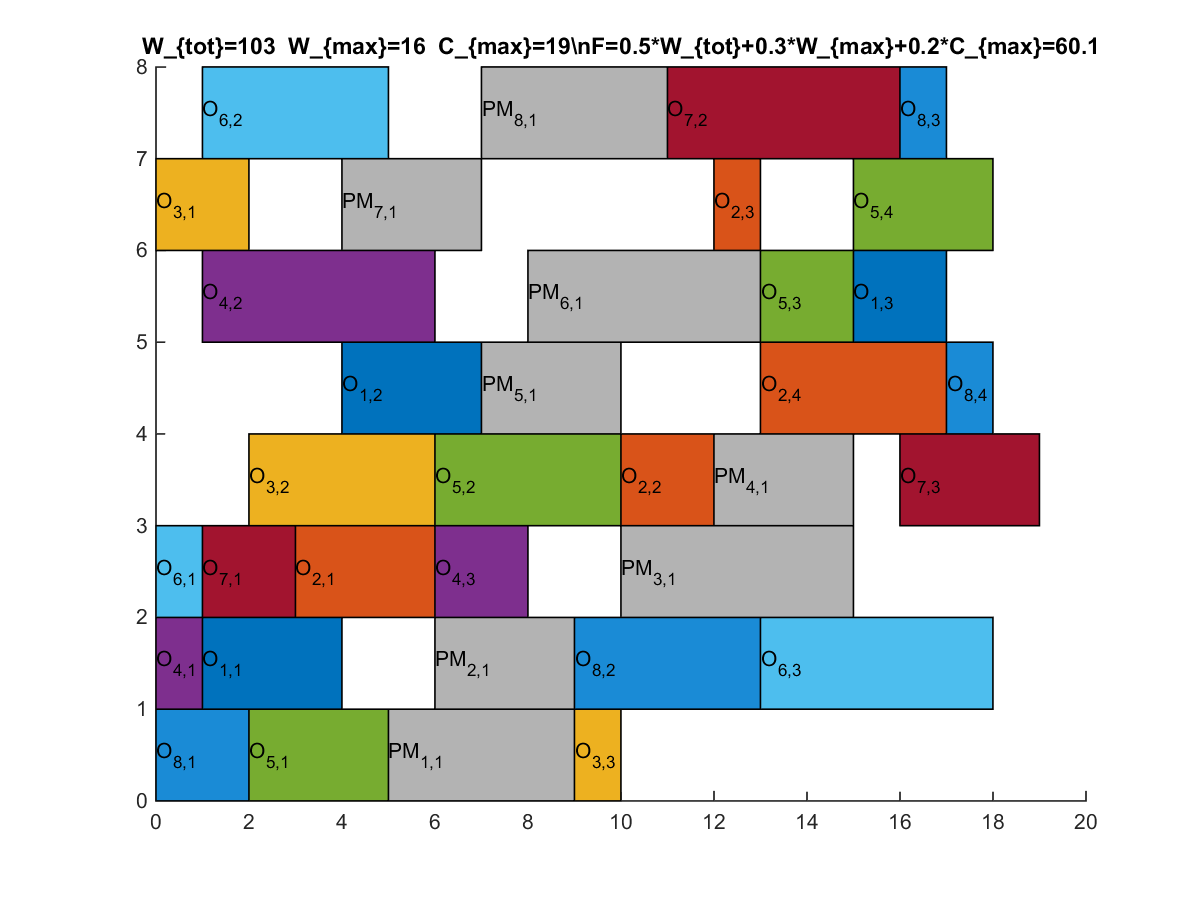
\includegraphics[width=0.8\textwidth]{img/results8x8_F050302.png}
  \caption{$8 \times 8$ $F(0.5;0.3;0.2)$ : $(W_t, W_{max}, C_{max}) = (40; 10; 15)$}
\end{figure}
\begin{figure}
  \centering
  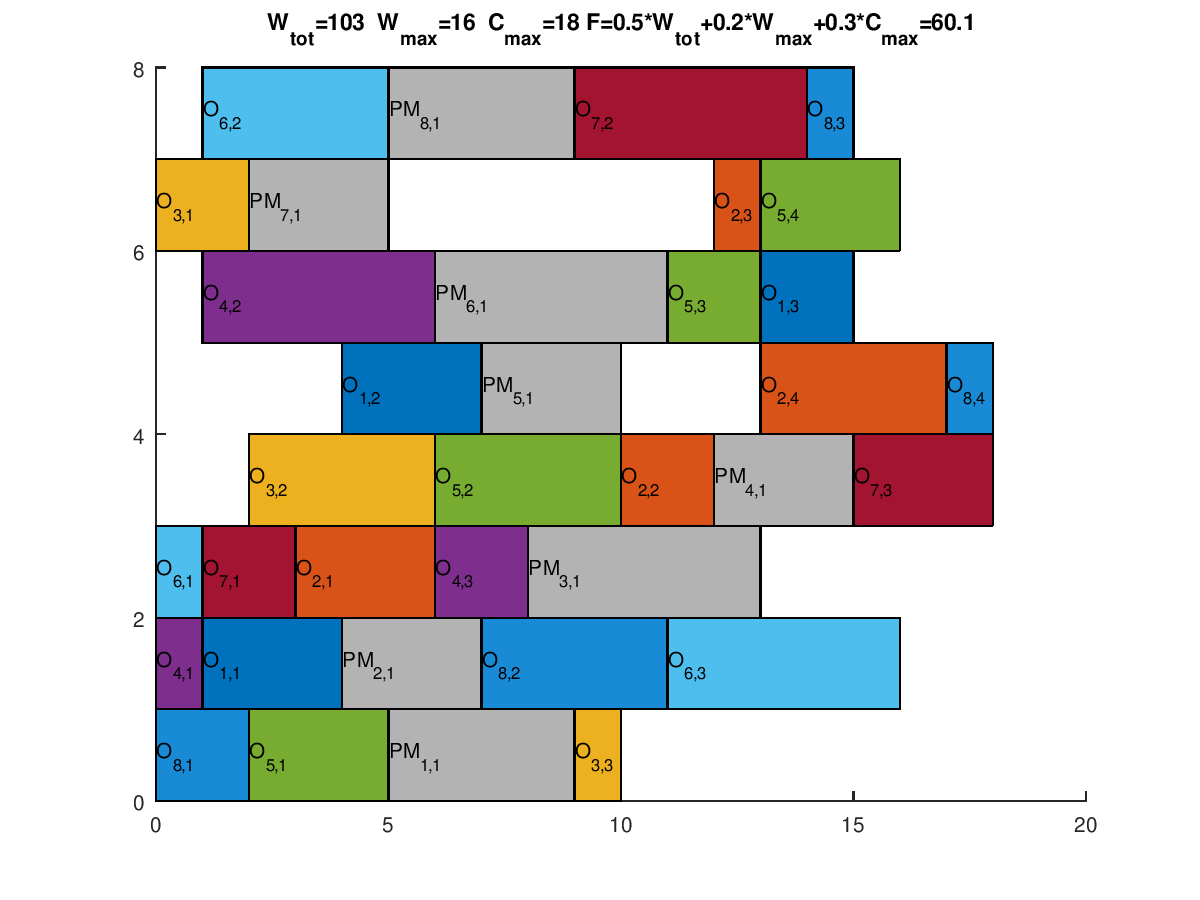
\includegraphics[width=0.8\textwidth]{img/results8x8_F050203.png}
  \caption{$8 \times 8$ $F(0.5;0.2;0.3)$ : $(W_t, W_{max}, C_{max}) = (40; 10; 15)$}
\end{figure}
\begin{figure}
  \centering
  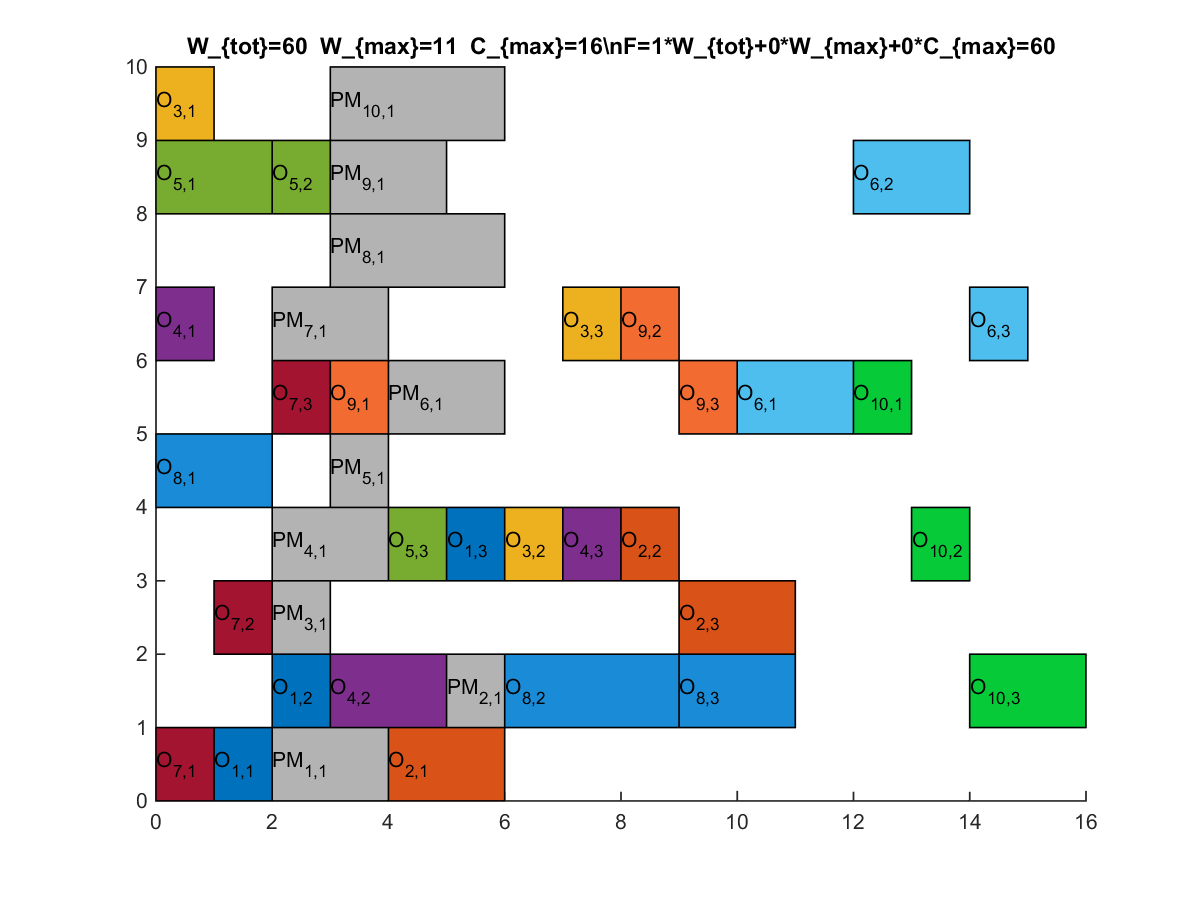
\includegraphics[width=0.8\textwidth]{img/results10x10_Wtot.png}
  \caption{$10 \times 10$ $W_{t}$ : $(W_t, W_{max}, C_{max}) = (60; 11; 16)$}
\end{figure}
\begin{figure}
  \centering
  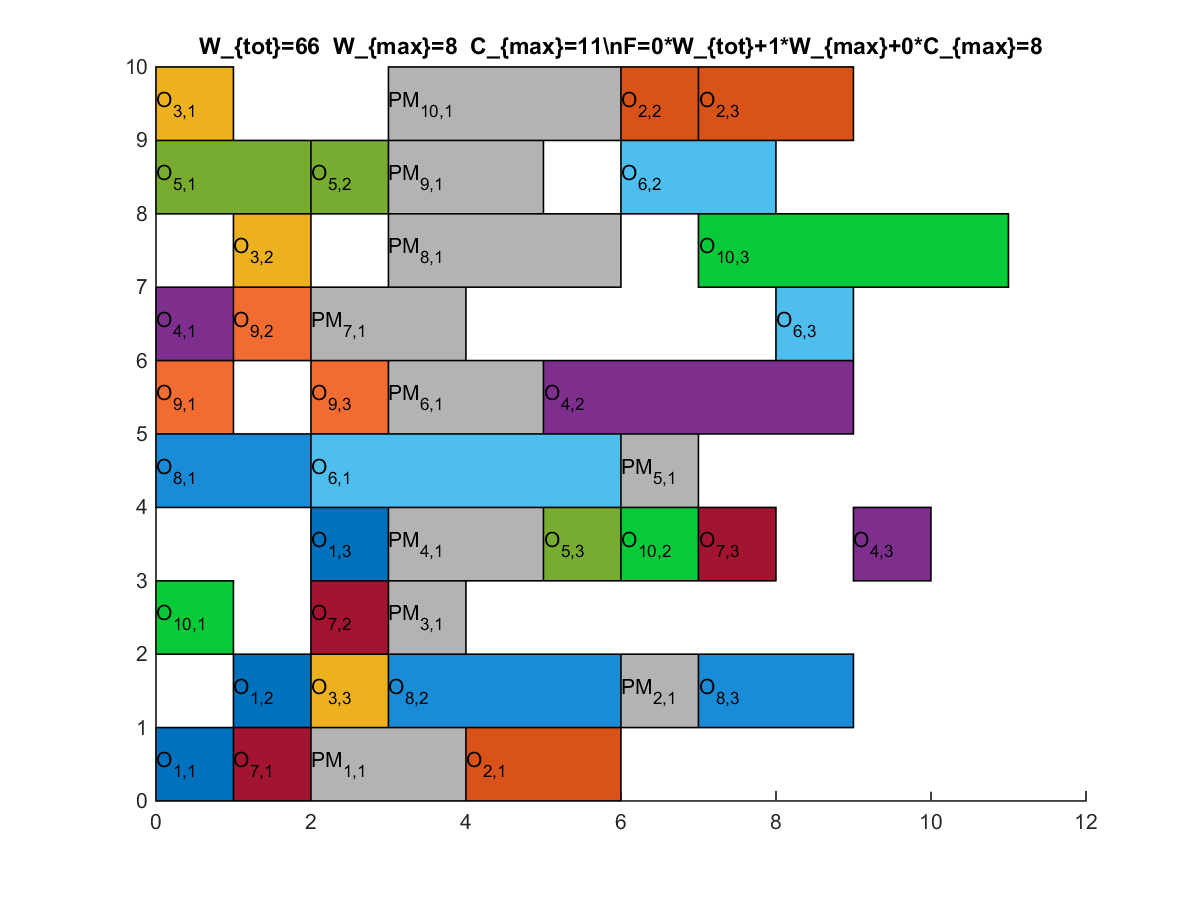
\includegraphics[width=0.8\textwidth]{img/results10x10_Wmax.png}
  \caption{$10 \times 10$ $W_{max}$ : $(W_t, W_{max}, C_{max}) = (66; 8; 11)$}
\end{figure}
\begin{figure}
  \centering
  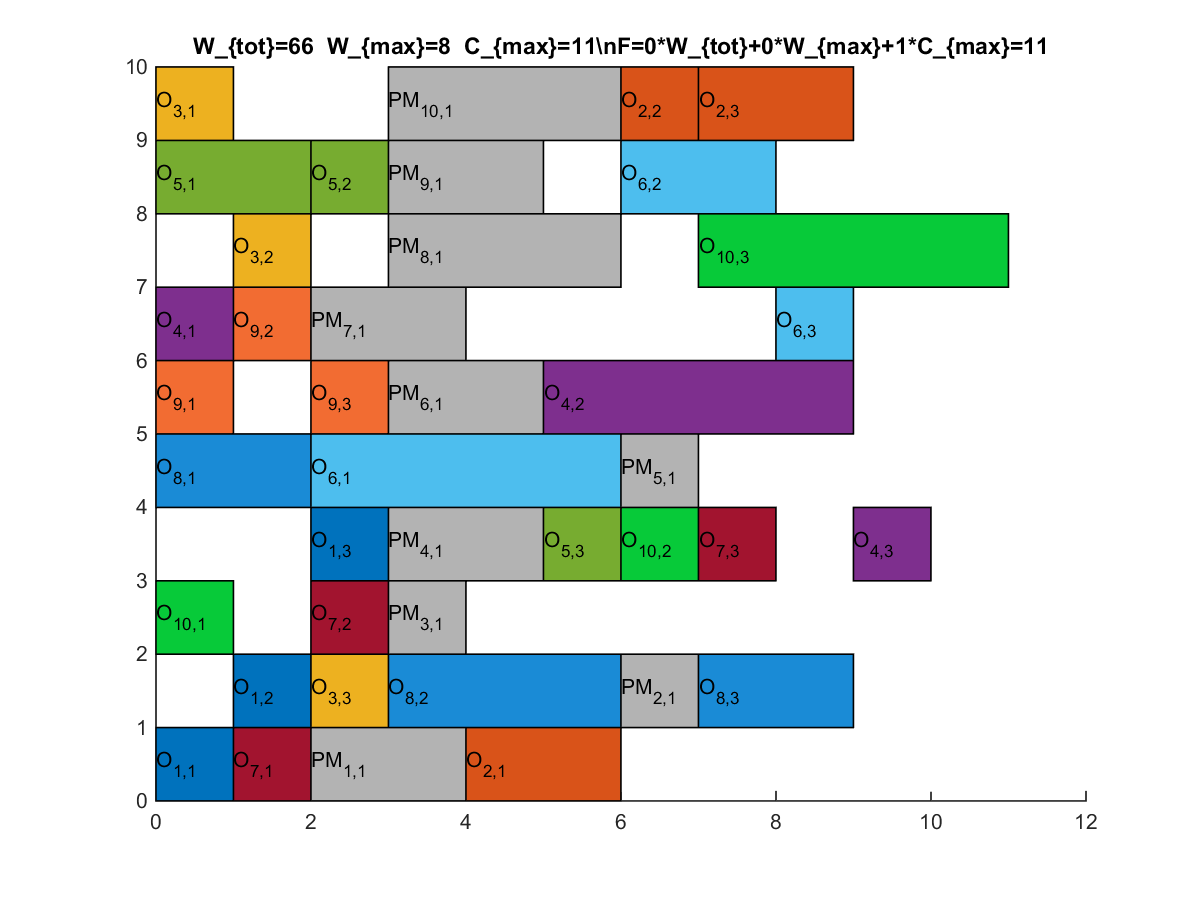
\includegraphics[width=0.8\textwidth]{img/results10x10_Cmax.png}
  \caption{$10 \times 10$ $C_{max}$ : $(W_t, W_{max}, C_{max}) = (66; 8; 11)$}
\end{figure}
\begin{figure}
  \centering
  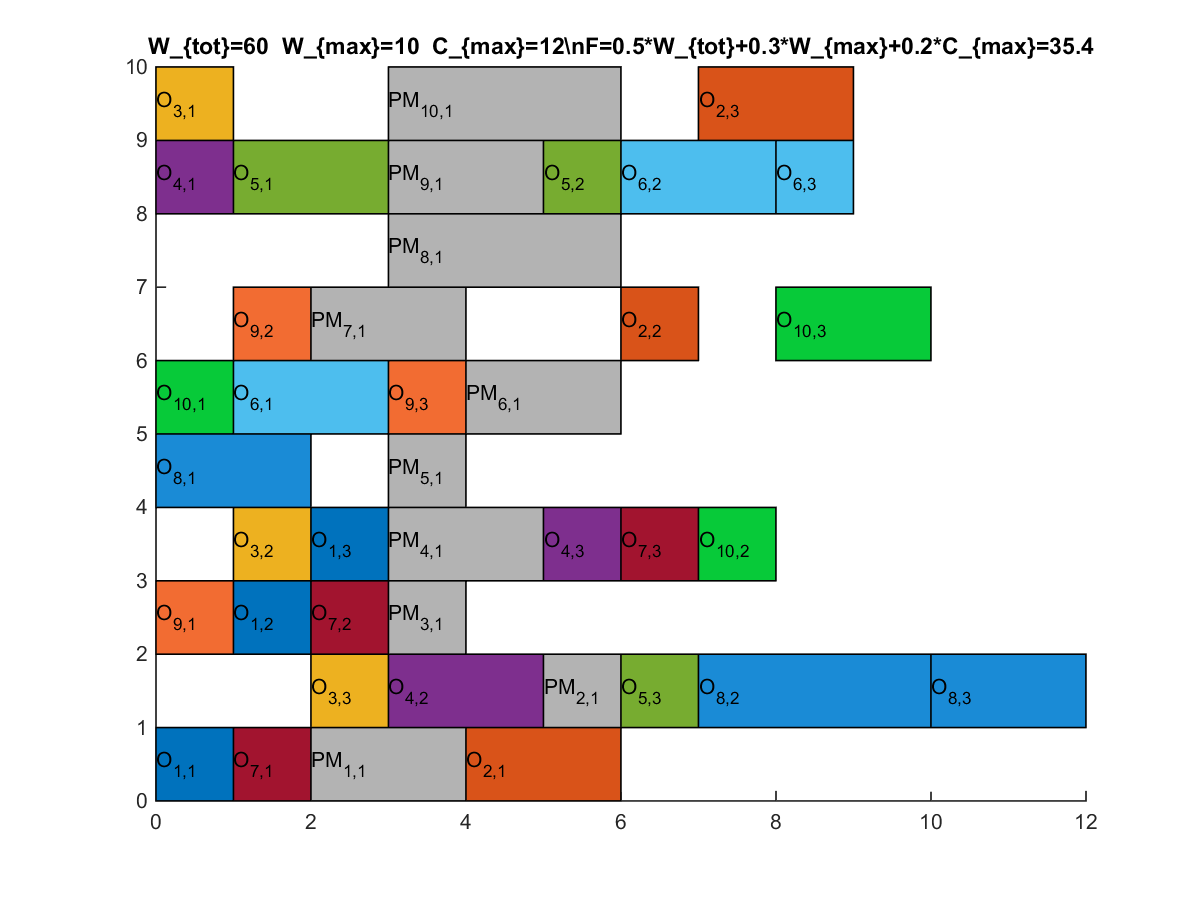
\includegraphics[width=0.8\textwidth]{img/results10x10_F050302.png}
  \caption{$10 \times 10$ $F(0.5;0.3;0.2)$ : $(W_t, W_{max}, C_{max}) = (60; 10; 12)$}
\end{figure}
\begin{figure}
  \centering
  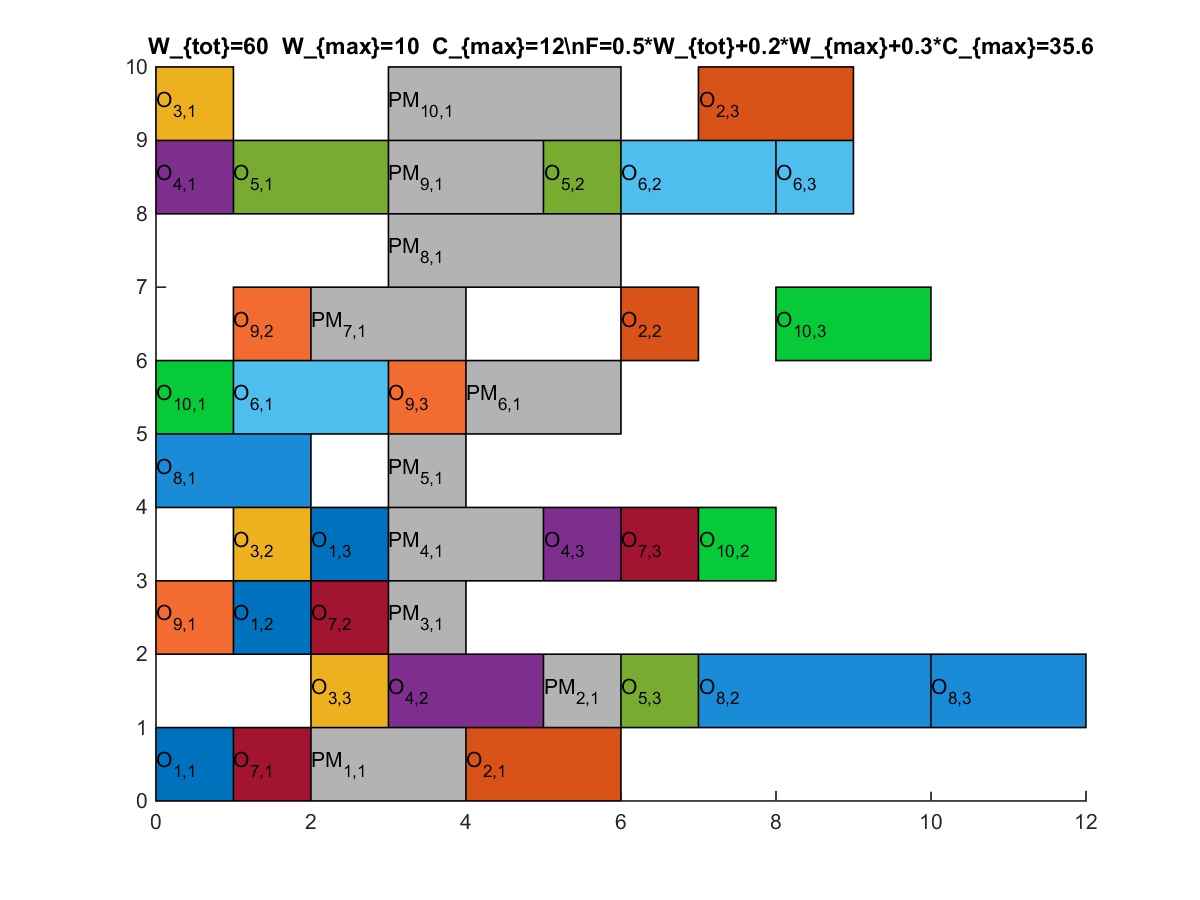
\includegraphics[width=0.8\textwidth]{img/results10x10_F050203.png}
  \caption{$10 \times 10$ $F(0.5;0.2;0.3)$ : $(W_t, W_{max}, C_{max}) = (60; 10; 12)$}
\end{figure}
\begin{figure}
  \centering
  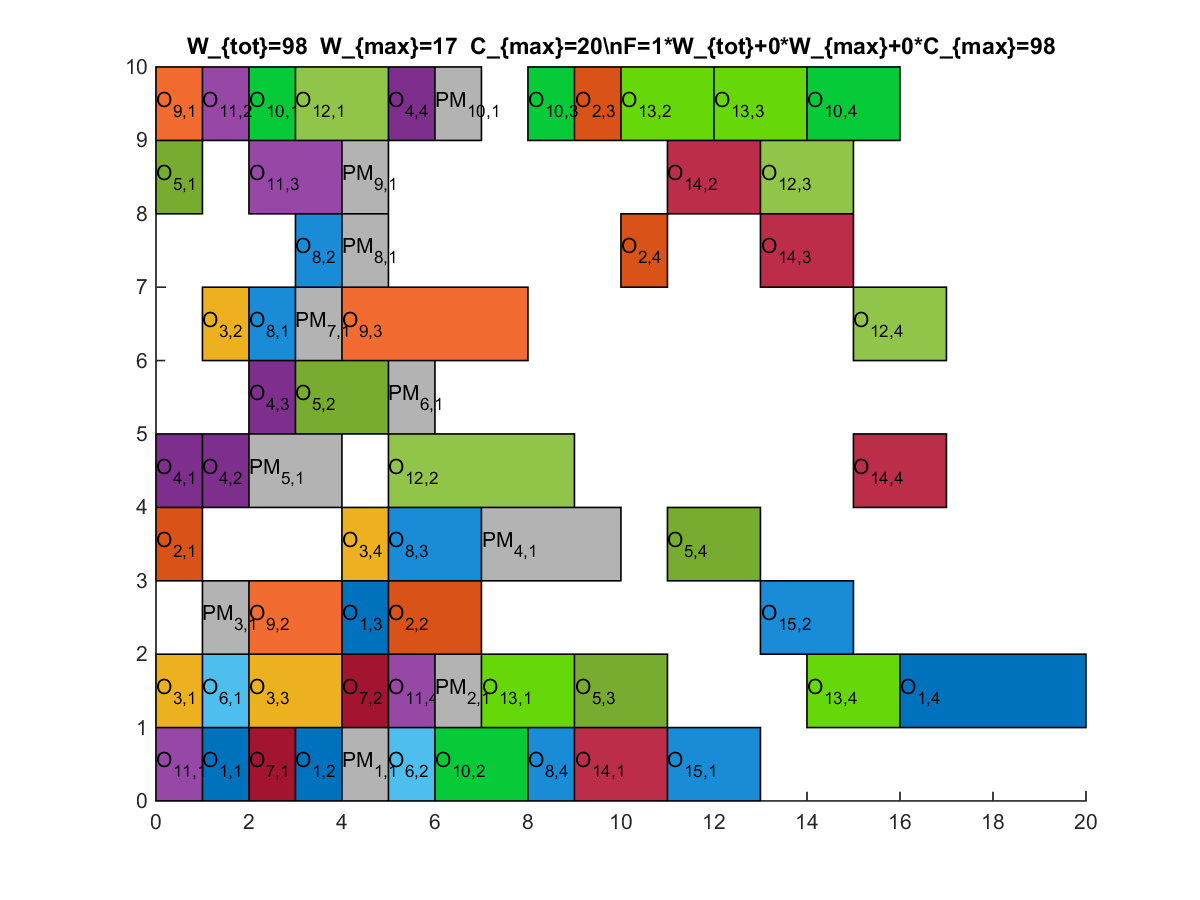
\includegraphics[width=0.8\textwidth]{img/results15x10_Wtot.png}
  \caption{$15 \times 10$ $W_{t}$ : $(W_t, W_{max}, C_{max}) = (98; 17; 20)$}
\end{figure}
\begin{figure}
  \centering
  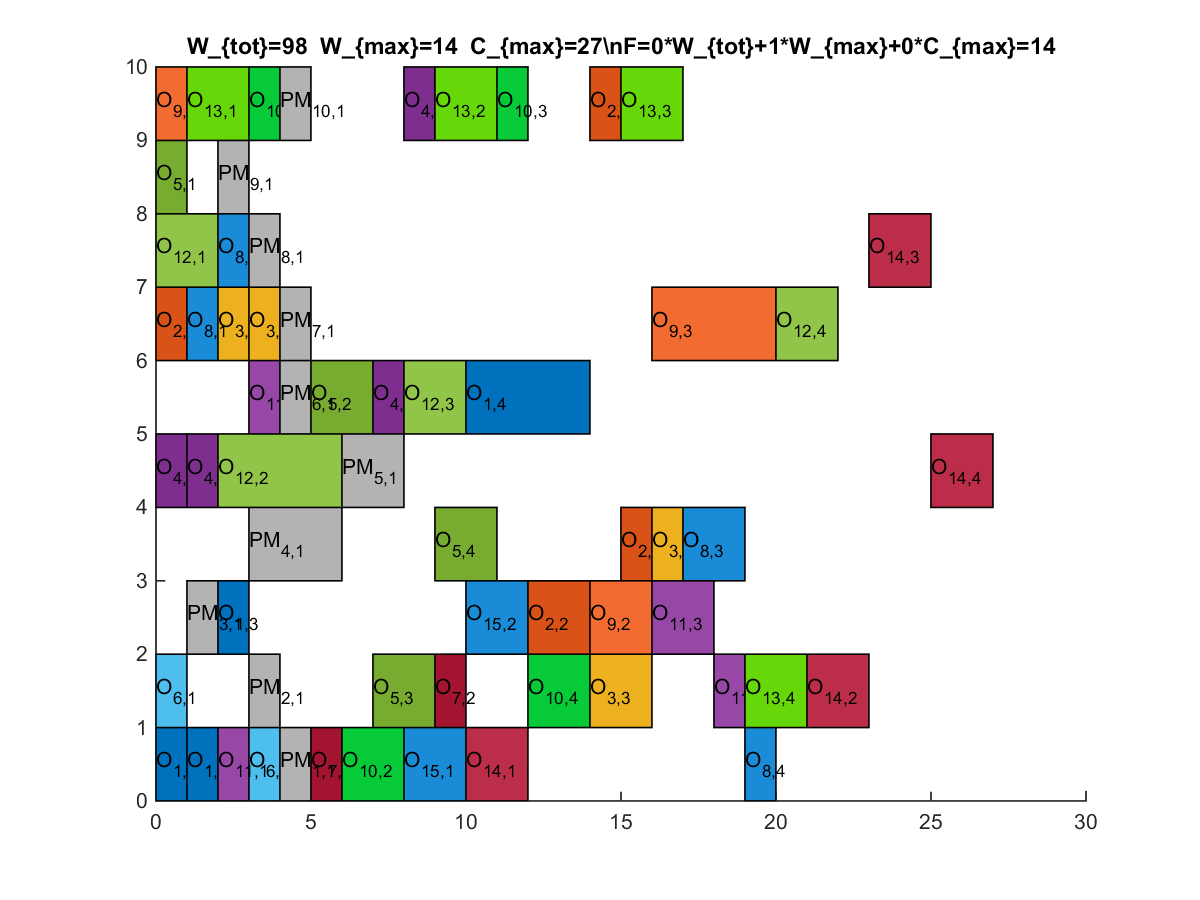
\includegraphics[width=0.8\textwidth]{img/results15x10_Wmax.png}
  \caption{$15 \times 10$ $W_{max}$ : $(W_t, W_{max}, C_{max}) = (98; 14; 27)$}
\end{figure}
\begin{figure}
  \centering
  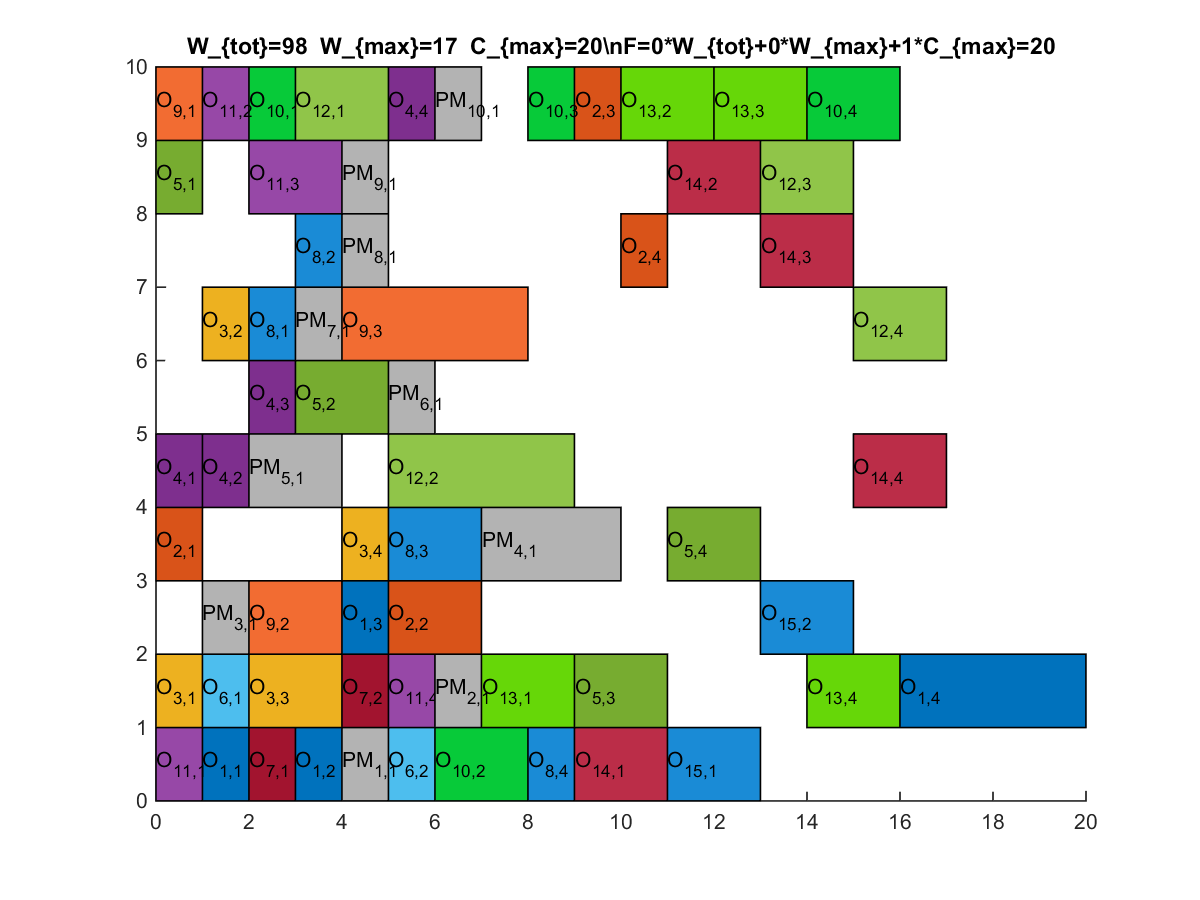
\includegraphics[width=0.8\textwidth]{img/results15x10_Cmax.png}
  \caption{$15 \times 10$ $C_{max}$ : $(W_t, W_{max}, C_{max}) = (98; 17; 20)$}
\end{figure}
\begin{figure}
  \centering
  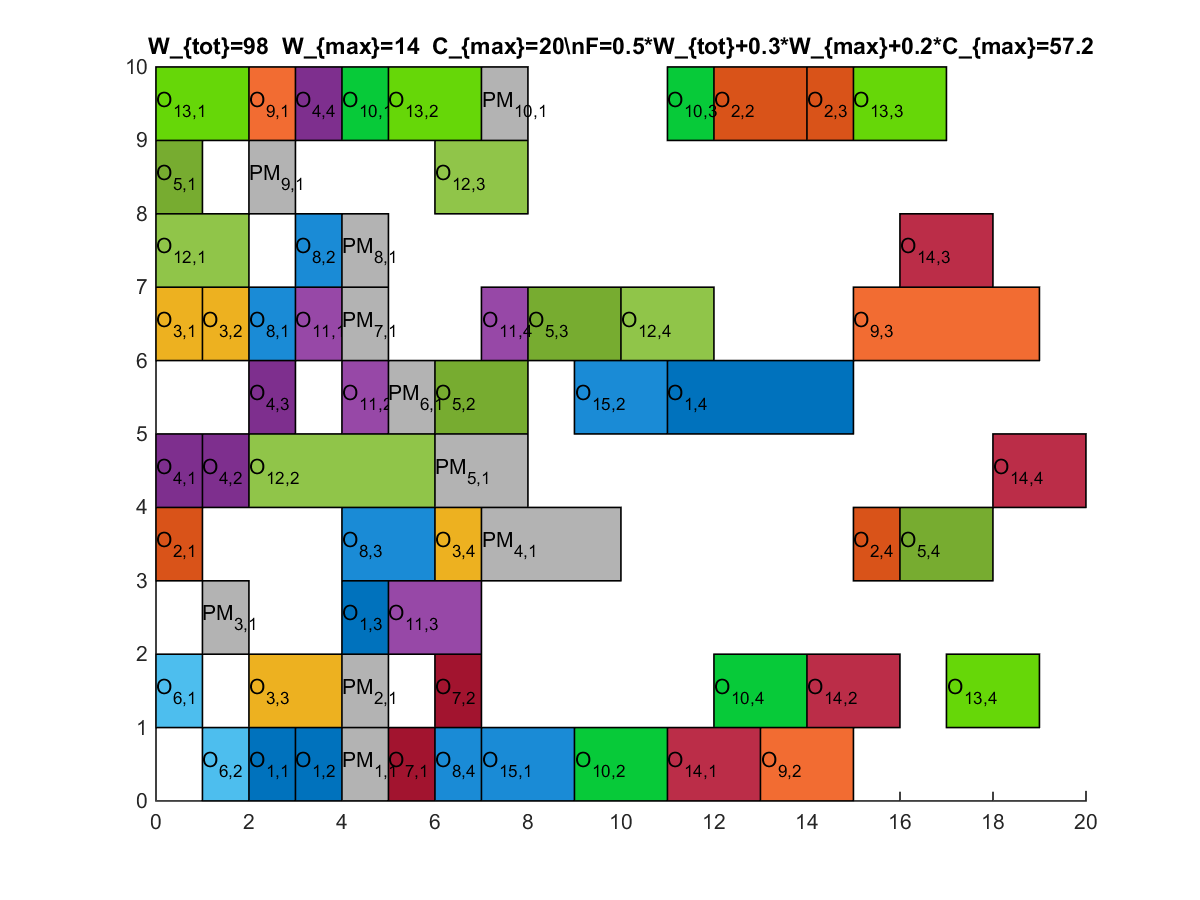
\includegraphics[width=0.8\textwidth]{img/results15x10_F050302.png}
  \caption{$15 \times 10$ $F(0.5;0.3;0.2)$ : $(W_t, W_{max}, C_{max}) = (98; 14; 20)$}
\end{figure}
\begin{figure}
  \centering
  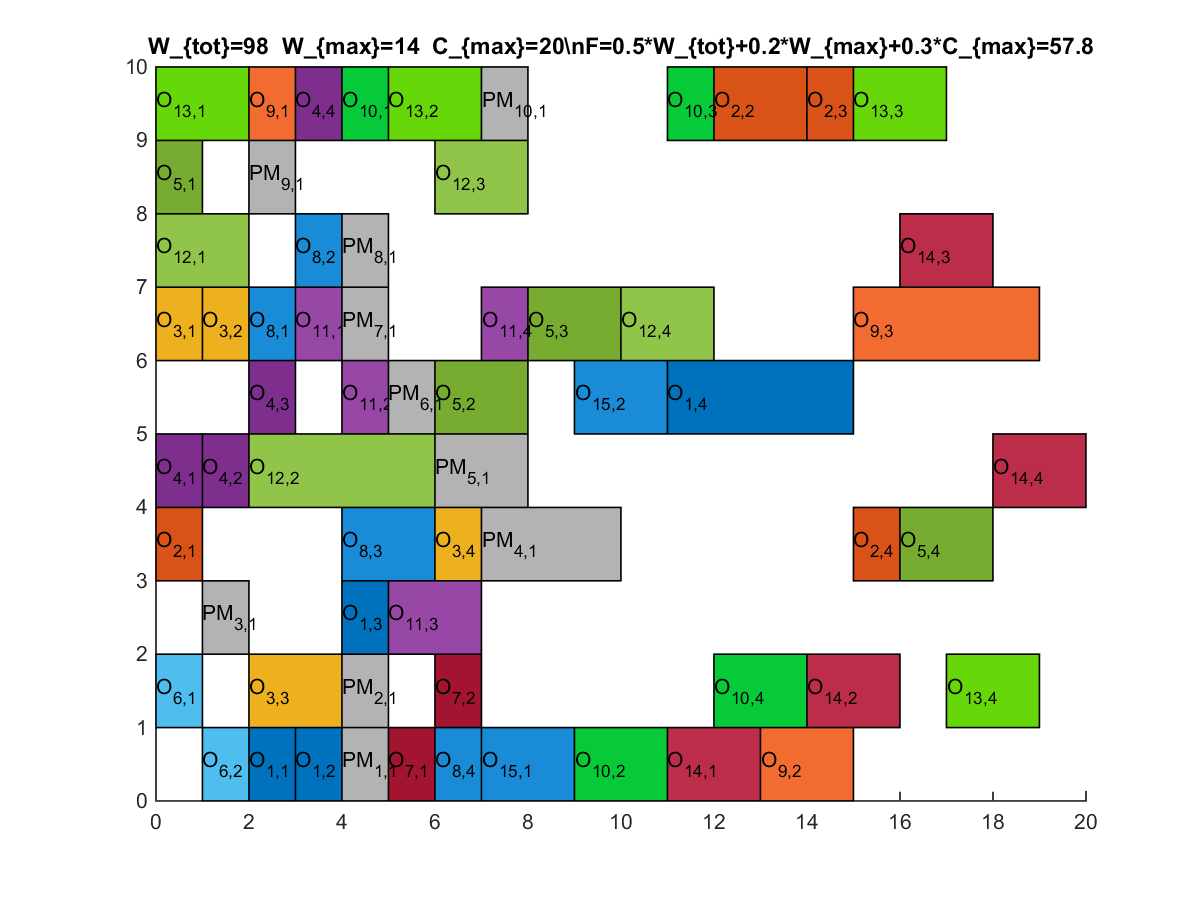
\includegraphics[width=0.8\textwidth]{img/results15x10_F050203.png}
  \caption{$15 \times 10$ $F(0.5;0.2;0.3)$ : $(W_t, W_{max}, C_{max}) = (98; 14; 20)$}
\end{figure}
\begin{figure}
  \centering
  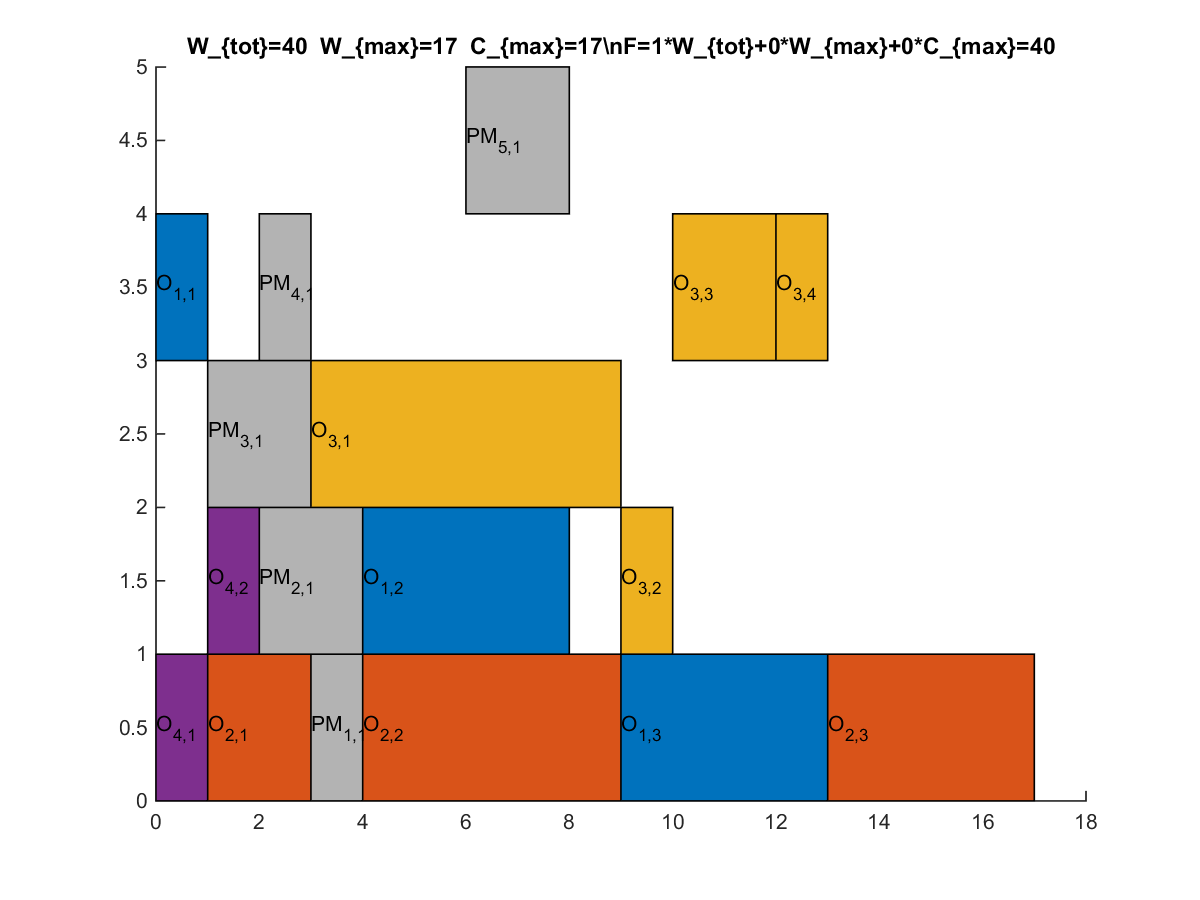
\includegraphics[width=0.8\textwidth]{img/results4x5_Wtot.png}
  \caption{$4 \times 5$ $W_{t}$ : $(W_t, W_{max}, C_{max}) = (40; 17; 17)$}
\end{figure}
\begin{figure}
  \centering
  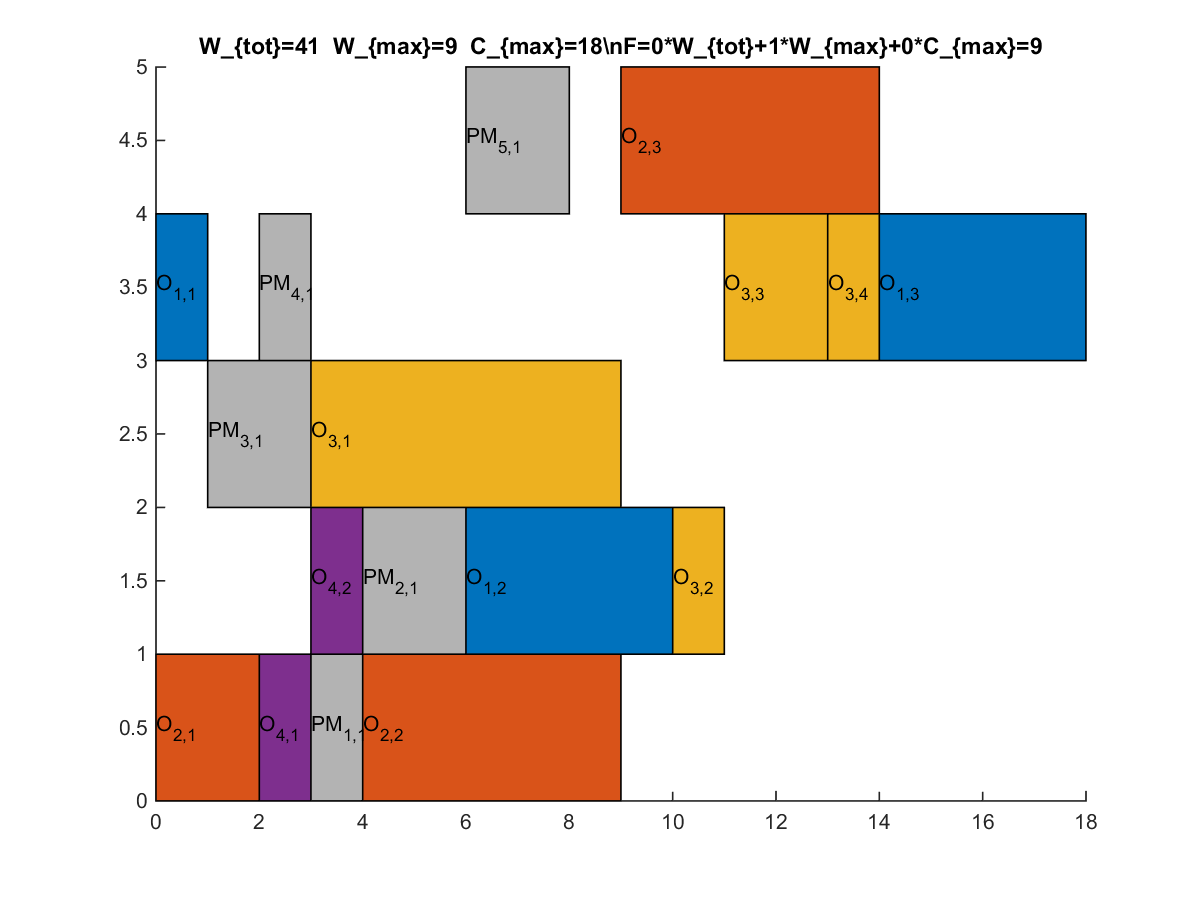
\includegraphics[width=0.8\textwidth]{img/results4x5_Wmax.png}
  \caption{$4 \times 5$ $W_{max}$ : $(W_t, W_{max}, C_{max}) = (41; 9; 18)$}
\end{figure}
\begin{figure}
  \centering
  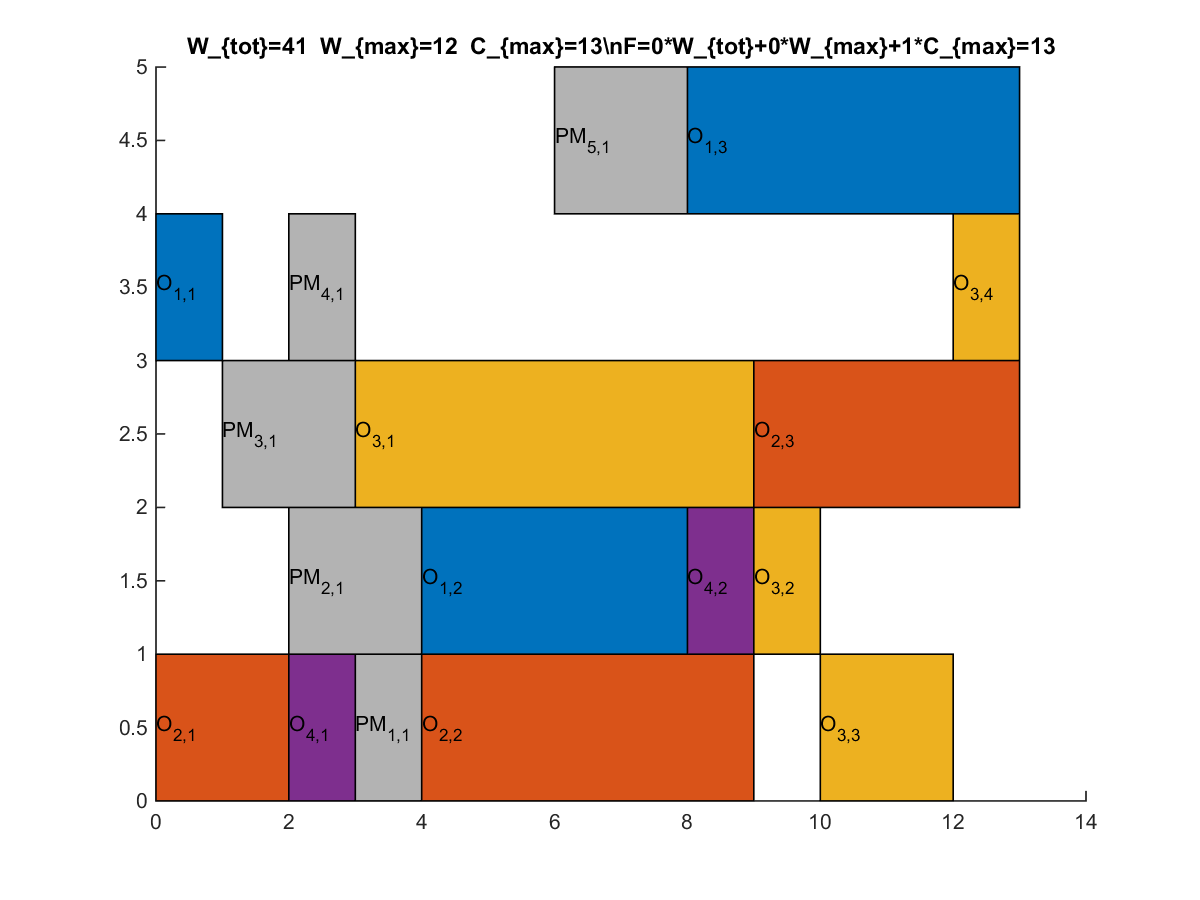
\includegraphics[width=0.8\textwidth]{img/results4x5_Cmax.png}
  \caption{$4 \times 5$ $C_{max}$ : $(W_t, W_{max}, C_{max}) = (41; 12; 13)$}
\end{figure}
\begin{figure}
  \centering
  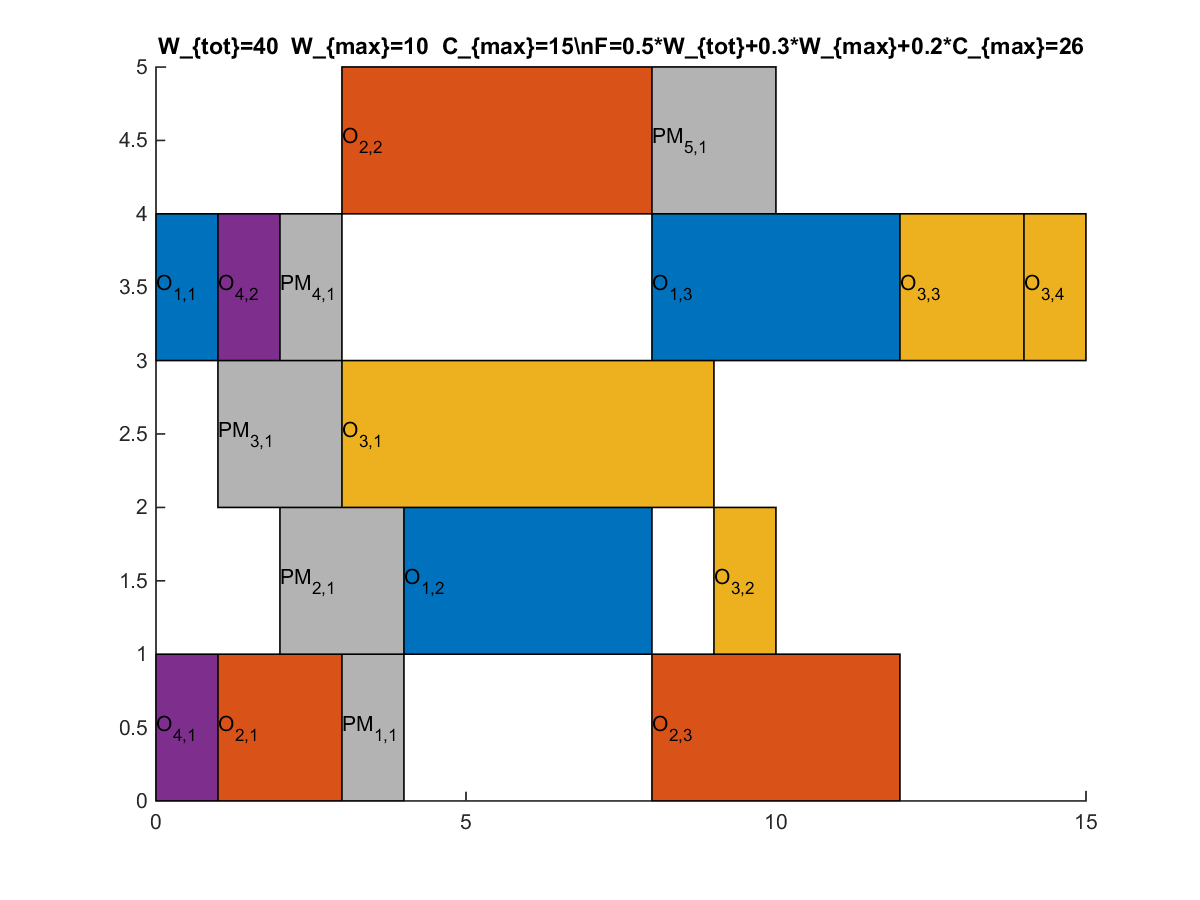
\includegraphics[width=0.8\textwidth]{img/results4x5_F050302.png}
  \caption{$4 \times 5$ $F(0.5;0.3;0.2)$ : $(W_t, W_{max}, C_{max}) = (40; 10; 15)$}
\end{figure}
\begin{figure}
  \centering
  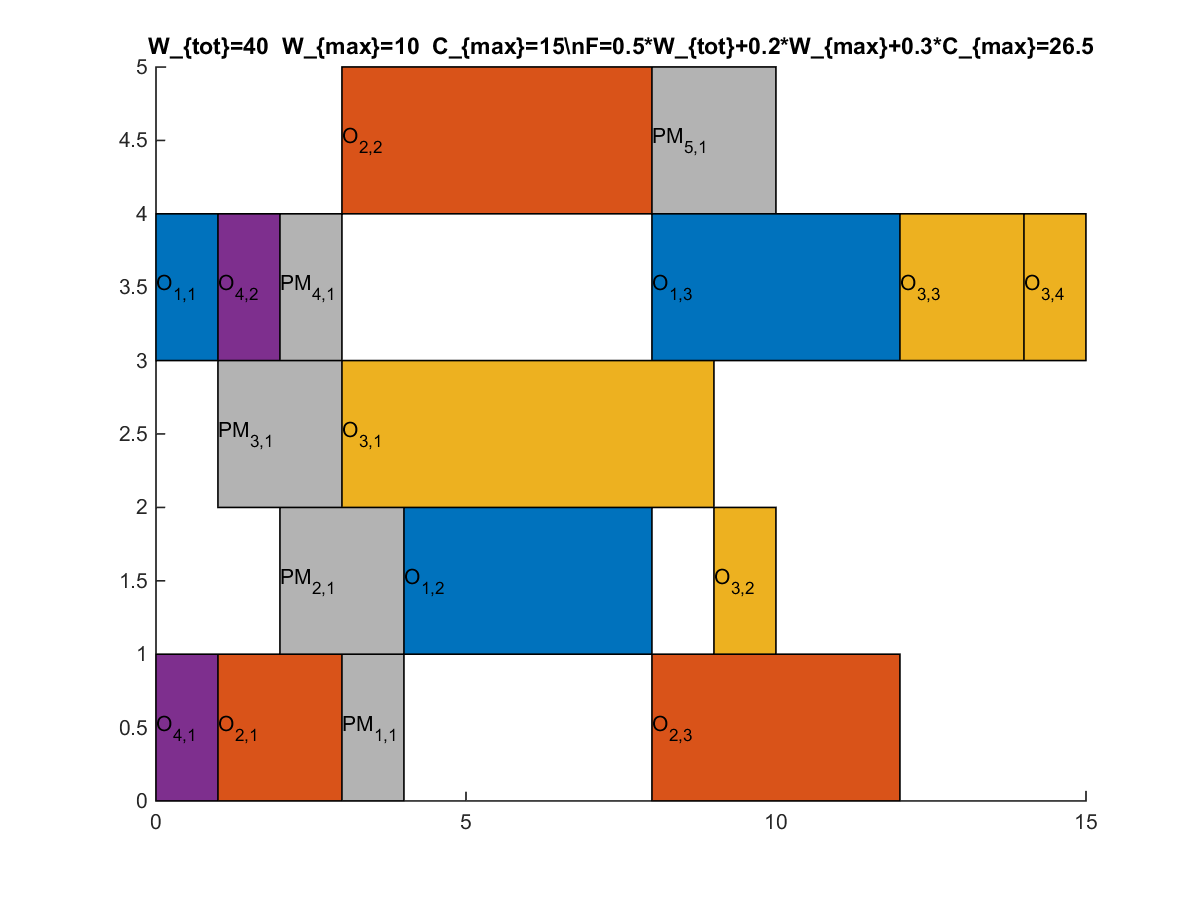
\includegraphics[width=0.8\textwidth]{img/results4x5_F050203.png}
  \caption{$4 \times 5$ $F(0.5;0.2;0.3)$ : $(W_t, W_{max}, C_{max}) = (40; 10; 15)$}
\end{figure}
\clearpage

\begin{thebibliography}{1}
\addcontentsline{toc}{section}{Références}
\bibitem{GRASP}
   Rajkumar, Muthukannan \& Asokan, P \& Vamsikrishna, V. (2010),
   \emph{A GRASP algorithm for flexible job-shop scheduling with maintenance constraints},
    International Journal of Production Research - INT J PROD RES. 48. 6821-6836. 10.1080/00207540903308969. 

\bibitem{GA1}
	F. Pezzella, G. Morganti, G. Ciaschetti,
	\emph{A genetic algorithm for the Flexible Job-shop Scheduling Problem},
	Computers \& Operations Research,
	Volume 35, Issue 10,
	2008,
	Pages 3202-3212,
	ISSN 0305-0548,
	https://doi.org/10.1016/j.cor.2007.02.014.
	(http://www.sciencedirect.com/science/article/pii/S0305054807000524)
	
\bibitem{GA2}	
	T. S. Chan, F \& Wong, T. C. \& Chan, LY. (2006). 
	\emph{Flexible job-shop scheduling problem under resource constraints}, 
	International Journal of Production Research - INT J PROD RES. 44. 2071-2089. 10.1080/00207540500386012. 
\end{thebibliography}
\end{document}